\section{Approach}
\label{sec:appro}
%In this section, we describe the general framework of our system to solve this problem. A running example will be given to illustrate the detail function of different parts of the system. 
%
%\subsection{Framework}

\begin{figure}[th!]
%\begin{figure}[H]
\centering
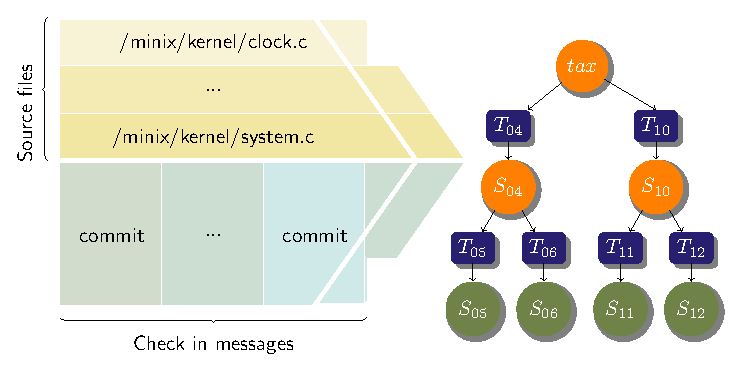
\epsfig{file=figure/framework.eps, width=0.6\columnwidth}
\caption{System Framework}
\label{fig:frame}
\end{figure}

\figref{fig:frame} shows the framework of our fault-tolerant
information extraction system. The input of the system is
one or more medical images of the same format (but 
with some slight variations), possibly after preprocessing. Those images will then be processed by the OCR Engine and will be turned into files in XML form with spatial annotations. Descriptions about those images in ODL will also be created by users or specific graphical user interfaces.
% Those graphical user interfaces will  generate descriptions mentioned above automatically given some parameters, which means it will save lots of work by the users.

 
%\JY{
Next, we propose a fuzzy parser to match all the elements on 
the provided description with the text from the XML data. The 
parser takes in XML data and corresponding ODL description as inputs 
and produces the parsing results. The parsing results are in the form of 
parsing trees in which every leaf nodes contains both the description and 
the corresponding textual information.
The word "fuzzy" means that the parser we created can not only extract useful information from those 
descriptions and XML files, but can tolerate the errors of our inputs as well during the extracting process. 
%Specifically, it should be noticed that XML files and descriptions can be inaccurate to some extent since there may exist some spelling mistakes or inaccurate human descriptions in the content of those input files. That is to say, the fuzzy parser can provide possible candidate parsing results instead of getting nothing in order to tolerate the errors. The most suitable result will be selected from those candidates by using the scoring policy which we will specify later.    


After the fuzzy parsing process, a parsing tree is generated, in which some extracted textual 
information may contains some OCR errors. In order to correct these errors, we design an 
incremental correction process. 
After multiple images are parsed, our system will find some common OCR errors 
discovered in these images.  
Our system will provide the user with those common OCR errors, and expect 
the user to give possible corrections. 
These corrections would then be used in our correction model and hence improve our parser.
%Subsequent parsing will be conducted based on the new model and 
%hopefully will result in fewer errors.

%}

% Our fuzzy parser then takes the XML and
% the corresponding ODL description as inputs, and produces the
% parsing result, which contains extracted values and possible 
% errors generated during parsing. 

% When multiple images are parsed,
% the system may direct the user to the common errors discovered in these
% images, which may be due to the same hardware, and prompt the user for
% possible corrections. Such corrections would then be incorporated
% into a correction model which is merged with the fuzzy parser.
% Subsequent parsing will be conducted based on the new model and 
% hopefully will result in fewer errors.

% \JY{
% Talk about the key concept in the approaches
% Fuzzy parser
% Optimization strategy
% Parameter tunning
% Learning from past
% Image variety
% }

In next few subsections, we will present a running example, using
an ECG image, with
which we will explain the syntax and semantics of ODL, 
as well as the interactive human correction mechanism in this framework.
%The techniques developed in this section can be applied to 
%other types of semi-structured medical images as well.
%The main components of our system are as follows:
%\begin{enumerate}
%\item The OCR engine generates XML files which contain both the recoginized text and the corresponding coordinates information. 
%\item The fuzzy parser, which is automatically generated based on the image description, is used to parse the XML files and extract the information. 
%\item The fuzzy parser will suggest some errors for human to correct, after that the correction model which is used for fuzzy parsing will be updated based on the correction that human made.
%\end{enumerate}

\subsection{Running Example}
Our running example is the ECG image shown in \figref{fig:ecgexample2}. 
In this example, we are interested in extracting the time, the measurements, 
and some basic diagnoses, all highlighted in the bright red ovals.
Fragments of the XML results coming out of the OCR engine are shown 
in \figref{fig:ocrre}. In addition, spatial coordinates for different 
OCR units, like paragraphs, lines and words, are recorded as values  
for the ``title'' attribute in XML. 

%There are numerous ways to describe the image using ODL.
%One of the descriptions, in concrete syntax, is shown in 
%\figref{fig:description}. 
Our discussion on the ODL language
will use the abstract syntax instead of concrete syntax. 
The abstract syntax of running example
is shown in \figref{fig:absdes}. 
%\JY{
In the description, 
{\em Osource} is the root description for the entire data of interest. 
Many types are used in the defination of {\em Osource} object to represent 
different forms of the textual information, for example, {\em Ostruct} is a type that 
represents the information with multiple fileds, and {\em Ounion} is a 
type that represents the enumerable information. 
%}
% {\em Ostruct} represents a structure
% of multiple fields. {\em Ounion} represents alternatives, while {\em Osource}
% is the root description of the entire data of interest.

%% \begin{figure}[ht]
% \centering
% \subfigure[]{
% \label{fig:subfig:a}
% \begin{minipage}[b]{0.2\textwidth}
\newsavebox{\thirdlisting}
\begin{lrbox}{\thirdlisting}% Store first listing
\small
\begin{lstlisting}[basicstyle=\tiny,]
*$Ounion$* month_str{
    "Jan"; "Feb"; "Mar"; 
    "Apr"; "May"; "Jun"; 
    "Jul"; "Aug"; "Sept";
    "Oct"; "Nov"; "Dec";
};

*$Ounion$* month_t{
    *$Oint$*(1,12)  num;
    month_str str;
};

*$Ostruct$* time_t{
    *$Oint$*(1,31)  day;
    "-";
    month_t month;
    "-";
    *$Oint$*()    year;
};

*$Ostruct$* triple_t{
    "Vent. rate";
    *$hskip$*(\s)   skip;
    *$Oint$*(60,100)    x;
    "bpm";
};
\end{lstlisting}
\end{lrbox}
% \end{minipage}
% }
% \hspace[1in]
% \subfigure[]{
% % \label{fig:subfig:b}
% % \begin{minipage}[b]{0.2\textwidth}
\newsavebox{\forthlisting}
\begin{lrbox}{\forthlisting}
\begin{lstlisting}[basicstyle=\tiny,]
*$Ounion$* inter_t{
    "Normal ECG";
    "Abnormal ECG";
};

*$Ostruct$* parameter_t{
    *$Oint$*()  p1;
    "Hz";
    *$Ofloat$*(3, 1)    p2;
    "mm/s";
    *$Ofloat$*(3, 1)    p3;
    "mm/mV";
};

*$Osource$* *$Ostruct$* entry_t{
    time_t(<_,_,_,0.3l>)  time;
    triple_t(<0.1w,_,0.5w,_>)  tri;
    inter_t(<tri.x1,tri.y0,_,_>)  i;
    *$vskip$*(\n)[]  skipline;
    parameter_t(<_,_,_,_>)  para;
};
*\vspace{8.5 mm}*
\end{lstlisting}
\end{lrbox}
% % \end{minipage}
% }

\begin{figure}[th]
\centering
\subfloat{
% \label{fig:description:a}
\scalebox{0.6}{\usebox{\thirdlisting}}
}
% \hfill
\subfloat{
% % \label{fig:description:b}
\scalebox{0.6}{\usebox{\forthlisting}}
}
\caption{ODL Description in Surface Syntax}
\label{fig:description}
\end{figure}

% \lipsum[2]

%% \begin{figure}[ht]
% \centering
% \subfigure[]{
% \label{fig:subfig:a}
% \begin{minipage}[b]{0.2\textwidth}
\newsavebox{\absflisting}
\begin{lrbox}{\absflisting}% Store first listing
\begin{lstlisting}[basicstyle=\tiny,]
    {
        {
            day(int, 1, 31),
            "-",
            {
                num(int, 1, 12) |
                {
                    "Jan" | "Feb" | "Mar" |
                    "Apr" | "May" | "Jun" |
                    "Jul" | "Aug" | "Sept" |
                    "Oct" | "Nov" | "Dec"
                } as str
            } as month,
            "-",
            year(int)
        }(<0.0w,0.0h,1.0w,0.3h>) as time,

        {
            "Vent. rate",
            *$hskip$* \t,
            vr(int, 60, 100),
            "bpm",
        }(<0.1w,0.0h,0.5w,1.0h>) as triple,
\end{lstlisting}
\end{lrbox}

% \newsavebox{\absflisting}
% \begin{lrbox}{\absflisting}% Store first listing
% % \fontsize{6pt}{7pt}\selectfont
% \begin{lstlisting}
%     {

%         {
%             day(int, 1, 31),
%             "-",
%             {
%                 num(int, 1, 12) |
%                 {
%                     "Jan" | "Feb" |
%                     "Mar" | "Apr" |
%                     "May" | "Jun" |
%                     "Jul" | "Aug" |
%                     "Sept" | "Oct" |
%                     "Nov" | "Dec"
%                 }
%             }
%             "-",
%             year(int)
%         }(<_,_,_,0.3l>),

%         {
%             "Vent. rate",
%             *$hskip$* \s,
%             x(int, 60, 100),
%             "bpm",
%         }(<0.1w,_,0.5w,_>) as triple,
% \end{lstlisting}
% \end{lrbox}


\newsavebox{\absslisting}
\begin{lrbox}{\absslisting}
% \fontsize{6pt}{7pt}\selectfont
\begin{lstlisting}[basicstyle=\tiny,]
        {
            "Normal ECG" |
            "Abnormal ECG"
        }(<0.3w,0.0h,1.0w,0.5h>) as inter,

        *$vskip$* \n list as skipline,

        {
            p1(int),
            "Hz",
            p2(float, 3, 1),
            "mm/s",
            p3(float, 3, 1),
            "mm/mV"
        } as para
    } as entry_t
\end{lstlisting}
\end{lrbox}
% % \end{minipage}

% \begin{figure}[ht]
% \centering
% \usebox\absflisting
% \caption{ODL description in abstract syntax.}
% \label{fig:running-odl-abstract}
% \end{figure}


\begin{figure}[ht]
\centering
\subfloat{
\scalebox{1.1}{\usebox{\absflisting}}
}
\subfloat{
\scalebox{1.1}{\usebox{\absslisting}}
}
\caption{The ODL description in abstract syntax.}
\label{fig:running-odl-abstract}
\end{figure}
% \lipsum[2]

% \begin{figure}
% \begin{lstlisting}
% time
%   day        F   "18"
%   "-"        F
%   month
%       str      F   "Jan"
%   "-"        F
%   year      F   "2012"

% triple
%   "Vent. rate"  F
%   skip1      F
%   x        F   "65"
%   "bpm"      F
%   skip2      F

% inter
%   "Abnormal ECG"   E   "Abnurrnal ECG"
  
% para
%   p1        E   "1oo"
%   "Hz"      F
%   p2        F   "25.0"
%   "mm/s"      F
%   p3        F   "1o.o"
%   "mm/mV"      F

% \end{lstlisting}
% \caption{Parsing Results}
% \label{fig:parsing result}
% \end{figure}


\begin{figure}[h]
\RawFloats
\begin{minipage}{0.45\textwidth}
%\subfloat{
% \label{fig:preresub:a}
\newsavebox{\prflisting}
\begin{lrbox}{\prflisting}% Store first listing
\begin{lstlisting}
time
  *$\langle$*day, F, "18"*$\rangle$*
  *$\langle$*"-", F*$\rangle$*
  month
    *$\langle$*str, F, "Jan"*$\rangle$*
  *$\langle$*"-", F*$\rangle$*
  *$\langle$*year, F, "2012"*$\rangle$*

triple
  *$\langle$*"Vent.rate", F*$\rangle$*
  *$\langle$*skip1, F*$\rangle$*
  *$\langle$*x, F, "65"*$\rangle$*
  *$\langle$*"bpm", F*$\rangle$*
  *$\langle$*skip2, F*$\rangle$*
\end{lstlisting}
\end{lrbox}

\newsavebox{\prslisting}
\begin{lrbox}{\prslisting}% Store first listing
\begin{lstlisting}
inter
  *$\langle$*"Abnormal ECG", F*$\rangle$*

para
  *$\langle$*p1, E, "15o"*$\rangle$*
  *$\langle$*"Hz", F*$\rangle$*
  *$\langle$*p2, F, "25.0"*$\rangle$*
  *$\langle$*"mm/s", F*$\rangle$*
  *$\langle$*p3, E, "1o.o"*$\rangle$*
  *$\langle$*"mm/mV", F*$\rangle$*
*\vspace{10 mm}*
\end{lstlisting}
\end{lrbox}

\scalebox{0.6}{\usebox\prflisting}
% \hfill
\hspace{7 mm}
\subfloat{
% \label{fig:preresub:b}
\scalebox{0.6}{\usebox{\prslisting}}}
\caption{Results of Our System}
\label{fig:parseresult}
\end{minipage}
\hfill
\begin{minipage}{0.45\textwidth}
\newsavebox{\absflisting}
\begin{lrbox}{\absflisting}% Store first listing
\begin{lstlisting}[basicstyle=\tiny,]
    {

        {
            day(int, 1, 31),
            "-",
            {
                num(int, 1, 12) |
                {
                    "Jan" | "Feb" | "Mar" | 
                    "Apr" | "May" | "Jun" | 
                    "Jul" | "Aug" | "Sept" | 
                    "Oct" | "Nov" | "Dec"
                }
            }
            "-",
            year(int)
        }(<_,_,_,0.3l>),

        {
            "Vent. rate",
            *$hskip$* \s,
            x(int, 60, 100),
            "bpm",
        }(<0.1w,_,0.5w,_>) as triple,

        {
            "Normal ECG" | 
            "Abnormal ECG"
        }(<triple.x1,triple.y0,_,_>),

        *$vskip$* \n list
        
        {
            p1(int),
            "Hz",
            p2(float, 3, 1),
            "mm/s",
            p3(float, 3, 1),
            "mm/mV"
        }(<_,_,_,_>)
    }
\end{lstlisting}
\end{lrbox}
\centering
% \subfloat
% \label{fig:absdes:a}
\scalebox{0.6}{\usebox\absflisting}
% \hfill
% \subfloat
% % \label{fig:absdes:b}
% {\usebox\absslisting}
\caption{ODL Description in Abstract Syntax}
\label{fig:absdes}
\end{minipage}
\end{figure}

% \begin{figure}[th]
% \centering
% \scalebox{1}{\usebox{\prslisting}}
% \caption{Results of Our System}
% \label{fig:parseresult}
% \end{figure}


% \KZ{Make the concrete syntax, abstract syntax figs double column and more
% compact.}

% in detail and notions

Those descriptions is then used as input for a fuzzy parser 
that produces a parsing representation, as shown in \figref{fig:parseresult}. 
If the system detects a popular OCR error, it may prompt the user for a
manual correction.
% For example, our system detects an error associated with
%variable $p1$ (the Hz value at the bottom of \figref{fig:ecgexample2}). In
%this case, ``150'' has been recognized as ``15o'' by the OCR.
%It prompts the user for a correction. If the user edits 
%``15o'' changing it to ``150,'' the system learns there is a possibility for the number ``0'' 
%to be mistaken for the letter ``o'' in this type of image by this particular OCR engine.
%Subsequently, in the same image and for other images of the same type, 
%the system may automatically  correct similar errors, e.g., 
%the value for variable $p2$ from ``1o.o'' to ``10.0.'' 

